
\chapter{Statistical tools for Extreme Value Theory}\label{appA}

\section{Tails of the distributions}\label{app:tails}


\subsection*{Heavy-tailed} 

\begin{definition}[Heavy-tails]
The distribution of a random variable $X$ with distribution function $F$ is said 
to have a \emph{heavy} right \emph{tail} if 
\begin{equation}
\displaystyle{\lim_{n \to \infty}} \ e^{\lambda x} \ \text{Pr}\{X>x\}=\displaystyle{\lim_{n 
\to \infty}} \ e^{\lambda x} \bar{F}(x)=\infty , \ \quad \forall \lambda>0.
\end{equation}
\end{definition}
More generally, we can say that a random variable X has heavy tails if Pr$\{|X|>x\}\to 0$ at 
a polynomial rate. In this case, note that some of the moments will be undefined.

\begin{definition}[Fat-tails]
The distribution of a random variable $X$ is said to have a \emph{fat} \emph{tail} if
\begin{equation}
\displaystyle{\lim_{x \to \infty}} \ \text{Pr}\{X>x\}=x^{-\alpha}.
\end{equation}
\end{definition}

\begin{definition}[Long-tails]
The distribution of a random variable X with distribution function F is said to have a \emph{long} 
right \emph{tail} if $\forall t > 0$,
\begin{equation}
\displaystyle{\lim_{x \to \infty}} \ \text{Pr}\{X>x+t|X>x\}=1 \ \Leftrightarrow \ 
\bar{F}(x+t)\sim\bar{F}(x) \quad \text{as} \ x\to\infty.
\end{equation}
\end{definition}


\begin{definition}[Light-tails]
Conversely, we say that $X$ has \emph{light tails} or \emph{exponential tails} if its tails decay at an exponential rate, i.e. 
\begin{equation}
\displaystyle{\lim_{x \to \infty}} \ \text{Pr}\{|X|>x\}=e^{-x}
\end{equation}
\end{definition}
An intuitive example of a distribution with exponential tails such as the exponential distribution.


\section{Convergence concepts}\label{convconc}


\subsection*{Convergence in distribution}

\begin{definition}[Convergence in distribution]
We say that a sequence $X_n$ with df $F_n$ converges in distribution to $X$ with df $F$, if 
\begin{equation}
F_n(x):=\text{Pr}\big\{X_n\leq x\big\}\longrightarrow \text{Pr}\{X\leq x\}:=F(x),
\end{equation}
at all continuity points of $F$. 
\end{definition}
It means that, for large $n$, $\text{Pr}\{X_n\leq t\}\approx\text{Pr}\{X\leq t\}$.
We denote this by $X_n\stackrel{d}{\to}X$.


\subsection*{Convergence in probability}

\begin{definition}[Convergence in probability]
We say that a sequence $X_n$ \emph{converges to $X$ in probability} if, $\forall\epsilon>0$, 
\begin{equation}
\text{Pr}\Big\{|X_n-X|>\epsilon\Big\}\to 0, \qquad\quad n\to\infty.
\end{equation}
\end{definition}
Hence, it means that the probability of the differnece between $X_n$ and $X$ goes to 0 as $n$ is large.  We denote this by $X_n\stackrel{P}{\rightarrow}X$.

An example of application of this convergence is the \emph{Weak Law of Large Numbers}. 

\begin{theorem}\label{wlln}[Weak Law of Large Numbers]
Let a sequence of R.V. $\{X_i\}_{\text{iid}}$ be defined of the same probability space with mean $\mu$ and variance $\sigma^2<\infty$. Then, we know that the difference between $\bar{X}_n$  and $\mu$ will go to 0 in probability, i.e. $\bar{X}_n\stackrel{p}{\to}\mu$.
\end{theorem}

But this law actually makes a stronger convergence, following \citet{kolmogorov_foundations_1956}, that is an \emph{almost sure convergence}

\subsection*{Almost Sure Convergence} 

This is the type of stochastic convergence that is most similar to pointwise convergence known from elementary real analysis.

\begin{definition}[Almost Sure convergence]
We say that a sequence of random variables $X_n$ \emph{converges almost surely} (or with probability one) to $X$ if 
\begin{equation}
\text{Pr}\Big\{X_n=X\Big\}=1, \quad\qquad n\to\infty.
\end{equation}
\end{definition}
We can denote this by $X_n\stackrel{\text{a.s.}}{\rightarrow} X$. This means that the values of $X_n$ approach the value of $X$, in the sense that events for which $X_n$ does not converge to $X$ have probability 0.


Well other forms of convergence do exist, but these ones are the most important in regard to EVT. However, the reader may refer e.g. to \citet{lafaye_understanding_2009}  for more in-depth results.

\section{Varying functions}\label{app:varying}

\begin{definition}[Regularly varying function]
Let's consider the survival $\bar{F}$. We say that this survival function $\bar{F}$ is \textbf{regularly varying} with index $-\alpha$ if
\begin{equation}
\displaystyle{\lim_{x \to \infty}} \frac{\bar{F}(xt)}{\bar{F}(x)}=t^{-\alpha}, \qquad t>0. 
\end{equation}
We write it $\bar{F}\in R_{-\alpha}$.
\end{definition}

\begin{definition}[Slowly varying function]
We say that a function $f$ is \textbf{slowly varying} with index $-\alpha$ if
\begin{equation}
\displaystyle{\lim_{x \to \infty}} \frac{f(t x)}{f(x)}=1, \qquad t>0. 
\end{equation}
\end{definition}
We remark that a slowly varying function is a regularly varying function with index 0.



\section{Diagnostic Plots : Quantile and Probability Plots}\label{app:qqpp}

From \citet[pp.18-36]{beirlant_practical_1996}, together with the nice view of \citet[pp.36-37]{coles_introduction_2001}, we present two major diagnostic tools which aim at assessing the fit of a particular model (or distribution) against the real distribution coming from the data used to construct the model.
These are called the \emph{quantile-quantile} plot (or \emph{qq}-plot) and the \emph{probability} plot (or \emph{pp}-plot). 

These diagnostics are popular by their easy interpretation and by the fact that they can both have graphical (i.e. subjective, qualitative, quick) view but also a more precise (i.e. objective, quantitative, rigorous) analysis can be derived, for example from the theory of linear regression. 
\newline
For these two diagnostic tools, we use the order statistics as seen (\ref{ordereds}) but now we rather consider an \textbf{ordered sample} of independent \textbf{observations} :

\begin{equation} \label{ordersamp}
x_{(1)}\leq x_{(2)}\leq\dots\leq x_{(n)}
\end{equation}
coming from a population from which we fit the estimated model (distribution) $\hat{F}$ and where $x_{(1)}$ (resp. $x_{(n)}$) is thus the minimum (resp. maximum) observation in the sample. We also define the \textbf{empirical distribution function}
\begin{equation}\label{eq:emprdist}
\tilde{F}(x)=\frac{i}{n+1}, \qquad\quad x_{(i)}\leq x\leq x_{(i+1)}.
\end{equation}
$\tilde{F}$ is an estimate of the true distribution $F$ and hence, by comparing $\hat{F}$ and $\tilde{F}$, it will help us to know if the fitted model $\hat{F}$ is reasonable for the data.

\subsubsection*{Quantile plot} Given a ordered sample as in (\ref{ordersamp}), a \emph{qq-plot} consists of the locus of points 

\begin{equation}
\Bigg\{\bigg(\hat{F}^{\leftarrow}\Big(\frac{i}{n+1}\Big)\ ,\ x_{(i)}\bigg) \ : \ i=1,\dots,n\Bigg\}.
\end{equation}
This graphic compares the ordered quantiles $\hat{F}^{\leftarrow}\Big(\frac{i}{n+1}\Big)$ of the fitted model $\hat{F}$ against the ordered observed quantiles, i.e. the ordered sample from (\ref{ordersamp}).
We used the continuity correction $\frac{i}{n+1}$ to prevent problems at the borders.
Note that a disadvantage of Q–Q plots is that the shape of the selected
parametric distribution is no longer visible \cite{beirlant_statistics_2006}[pp.63]

\subsubsection*{Probability plot} Given the same sample in (\ref{ordersamp}), a \emph{probability plot} consists of the locus of points 

\begin{equation}
\Bigg\{\bigg(\hat{F}(x_{(i)})\ ,\ \frac{i}{n+1}\bigg) \ : \ i=1,\dots,n\Bigg\}.
\end{equation}
This graph compares the estimated probability of the ordered values $x_{(i)}$, thus from the fitted model $\hat{F}$, against the probability coming from the empirical distribution as in (\ref{eq:emprdist}). 

From these two graphical diagnostic tools, the interpretation is the same and we will consider that $\hat{F}$ fits well the data if the plot looks linear, i.e. the points of the plots lie close to the unit diagonal.

Besides the fact that the probability and the quantile plots contain the same information, they are expressed in a different scale. That is, after changing the scale to probabilities or quantiles (with probability or quantile transforms), one can gain a better perception and both visualizations can sometimes lead contradictory conclusions, especially in the graphical inspection. Using both is thus preferable to make our model's diagnostic more robust.

\chapter{Bayesian Methods}\label{appB}

\section{Algorithms}

\subsection{Metropolis–Hastings Algorithm}

The \emph{Metropolis–Hastings} algorithm is one of the first and of the pioneering algorithm discovered by \cite{hastings_monte_1970} to compute  MCMC for Bayesian analysis.

\begin{algorithm}[H]
	\SetAlgoLined
	\begin{enumerate}
		\item Pick a starting point $\theta_0$ and fix some number $N$ of simulations.
		\item \textbf{For} $t=1,\dots,N$ \quad \textbf{do}
		\begin{itemize}
			\item[(a)] Sample proposal $\theta_*$ from a proposal density $p_t(\theta_*|\theta_{t-1})$,
			\item[(b)] Compute the ratio
			\begin{equation*}
			r = \frac{\pi(\theta_*|\boldsymbol{x})\cdot p_t(\theta_{t-1}|\theta_*)}{\pi(\theta_{t-1}|\boldsymbol{x})\cdot p_t(\theta_*|\theta_{t-1})} = \frac{\pi(\theta_*)\cdot \pi(\boldsymbol{x}|\theta_*)\cdot p_t(\theta_{t-1}|\theta_*)}{\pi(\theta_{t-1})\cdot \pi(\boldsymbol{x}|\theta_{t-1})\cdot p_t(\theta_*|\theta_{t-1})}.
			\end{equation*}
			\item[(c)] Set 
			\begin{equation*}
			\theta_t= 			\begin{cases} \ \theta_* \qquad \text{with probability} \ \  \alpha=\min (r,1); \\
			\ \theta_{t-1} \ \quad \text{otherwise}.
			\end{cases}
			\end{equation*}
		\end{itemize}
	\end{enumerate}
	\caption{The Metropolis–Hastings Algorithm}
\end{algorithm}


This algorithm remains valid when $\pi$ is only proportional to a target density function and thus it can be used to approximate \ref{bayeseq} . 

Note that the proposal density is often chosen to be symmetric so that we will just sample under a "simple Metropolis" algorithm where $r$ is thus simplified to be only the ratio of the posterior densities, $r=\frac{\pi(\theta_*|\boldsymbol{x})\cdot }{\pi(\theta_{t-1}|\boldsymbol{x})}$.

We can shortly summarize the \emph{pros} and \emph{cons} this algorithm :

\begin{itemize}
	\item \emph{PROS} : Very easy to program and works even for relatively complex densities.
	\item \emph{CONS} : Can be very inefficient, in the sense that it will require lots of iterations before the stationary target distribution will be reached. This requires some tuning to the algorithm through 
\end{itemize}


\subsection{Gibbs Sampler}

The \emph{Gibbs Sampler} can be seen as a special case of the Metropolis-Hastings algorithm.
Suppose our parameter vector $\theta$ can be divided into $d$ subvectors $(\theta_1,\dots,\theta_d)$, and let's say in our case that each of these "subvectors" represent a single parameter, thus typically one of the three $(\mu,\sigma,\xi)$, for the simplest case so that $d=3$ in this model.
At each $t=1,\dots,N$, the Gibbs sampler samples the subvectors $\theta_t^{(j)}$ conditional on both the data $\boldsymbol{x}$ and the remaining subvectors $\theta_{t-1}^{(-j)}$ at their current values.
Therefore, we have $\theta_{t-1}^{(-j)}=\Big(\theta_t^{(1)},\dots,\theta_t^{(j-1)},\theta_{t-1}^{(j+1)},\dots,\theta_{t-1}^{(d)}\Big)$ and each $\theta_t^{(j)}$ is sampled from $\pi\Big(\theta^{(j)}|\theta_{t-1}^{(-j)},\boldsymbol{x}\Big)$. \\

\begin{algorithm}[H]
	\SetAlgoLined
	\begin{enumerate}
		\item Pick a starting point $\theta_0$ and fix some number $N$ of simulations.
		\item \textbf{For} $t=1,\dots,N$ \qquad \textbf{do} \\
		\quad \textbf{For} $j=1,\dots,d$ \qquad \textbf{do}
		\begin{itemize}
			\item[(a)] Sample proposal $\theta_*$ from a proposal density $p_{t,j}(\theta^{(j)}_*|\theta^{(j)}_{t-1})$,
			\item[(b)] Compute the ratio
			\begin{equation*}
			\begin{aligned}
				r = & \frac{\pi\Big(\theta^{(j)}_*|\theta_{t-1}^{(-j)},\boldsymbol{x}\Big)\cdot p_{t,j}\Big(\theta^{(j)}_{t-1}|\theta^{(j)}_*\Big)}{\pi\Big(\theta_{t-1}^{(j)}|\theta_{t-1}^{(-j)},\boldsymbol{x}\Big)\cdot p_{t,j}\Big(\theta^{(j)}_*|\theta_{t-1}\Big)} \\
				= & \frac{\pi\Big(\theta_t^{(1)},\dots,\theta_t^{(j-1)},\theta^{(j)}_*, \theta_{t-1}^{(j+1)},\dots,\theta_{t-1}^{(d)} \ | \ \boldsymbol{x}\Big)\cdot  p_{t,j}\Big(\theta_{t-1}^{(j)}|\theta_*^{(j)}\Big)}{\pi\Big(\theta_t^{(1)},\dots,\theta_t^{(j-1)},\theta^{(j)}_{t-1}, \theta_{t-1}^{(j+1)},\dots,\theta_{t-1}^{(d)}\ |\ \boldsymbol{x}\Big)\cdot  p_{t,j}\Big(\theta_{*}^{(j)}|\theta_{t-1}\Big)},
		\end{aligned}
			\end{equation*}
			\item[(c)] Set 
			\begin{equation*}
			\theta_t^{(j)}= 			\begin{cases} \ \theta_*^{(j)} \qquad \text{with probability} \ \  \alpha=\min (r,1); \\
			\ \theta_{t-1}^{(j)} \ \ \quad \text{otherwise}.
			\end{cases}
			\end{equation*}
		\end{itemize}
	\end{enumerate}
	\caption{PSEUDOCODE of the Gibbs Sampler}
\end{algorithm}
(better signs for conditional bar "|" !!!!!!!


This algorithm depends on being able to simulate from $\pi\Big(\theta^{(j)}|\theta_{t-1}^{(-j)},\boldsymbol{x}\Big)$ which is often impossible. However, one can use Metropolis-Hastings to $\pi\Big(\theta^{(j)}|\theta_{t-1}^{(-j)},\boldsymbol{x}\Big)$, giving the above.

A special case arise if one can simulate directly so that $r=1$, i.e. we take $p_{t,j}\big(\theta_*^{(j)}|\theta_{t-1}^{(j)}\big)=\pi\big(\theta_*^{(j)}|\theta_{t-1}^{(-j)},\boldsymbol{x}\big)$.
(The proposal $p_{t,j}(\cdot)$ is also often symmetric, i.e.
$p_{t,j}\big(\theta_*^{(j)}|\theta_{t-1}^{(j)}\big)= p_{t,j}\big(\theta_{t-1}^{(j)}|\theta_*^{(j)}\big)$. But it cannot be simplified in the equation. )

It is important for our tasks to tune the average probability of acceptance to be roughly between 0.4 and 0.5 (see e.g. \citet[chapter 11]{gelman_bayesian_2013} ) so that the so-generated markov-chain has desirable properties. This is doneby setting the standard deviation $\sigma{(j)}$ of the univariate normal distribution taken for $p_{t,j}\big(\theta_*^{(j)}|\theta_{t-1}^{(j)}\big)$. Whereas our $\theta{(j)}$ are (often?) univariate, it is difficult to set each $\sigma^{(j)}$ to achieve average acceptance probabilities for all parameters. We will then use a trial-and-error approach.

Note also the increase of complexity with this sampler compared to the Metropolis-Hastings, where the nested loop implies that there are $d$ iterations with each simulation.


\emph{pros} and \emph{cons} : 

\begin{itemize}
	\item \emph{PROS} : Easy to program and, for some problems, it can also be very efficient. It is a pleasant way to split multidimensional problems into simpler (typically univariate) densities.
	\item \emph{CONS} : Sometimes hard to compute analytically the conditional distributions. Not all densities can be split into pleasant conditionals equations.
\end{itemize}



\subsubsection*{Metropolis-within-Gibbs?}



\subsection{Hamiltonian Monte Carlo}

\url{http://deeplearning.net/tutorial/hmc.html#hmc} \\

A difficulty we have faced and that we would like to point out for GEV models is (see p.316-317 STAN manual) t




"Most of the computation [in Stan] is done using Hamiltonian Monte Carlo. HMC requires some tuning, so Matt Hoffman up and wrote a new algorithm, Nuts (the “No-U-Turn Sampler”) which optimizes HMC adaptively. In many settings, Nuts is actually more computationally efficient than the optimal static HMC! "

The \emph{Hamiltonian Monte Carlo} (HMC)

"The Hamiltonian Monte Carlo algorithm starts at a specified initial set of parameters
theta; in Stan, this value is either user-specified or generated randomly. Then, for a given
number of iterations, a new momentum vector is sampled and the current value of
the parameter $\theta$ is updated using the leapfrog integrator with discretization time 
and number of steps L according to the Hamiltonian dynamics. Then a Metropolis
acceptance step is applied, and a decision is made whether to update to the new state
(theta*; rho*) or keep the existing state" \cite{stan_stan_2016}



\cite{Hartmann_bayesian_2016} have demonstrated in similar application that HMC  (and Riemann manifold HMC) are much more computationally efficient than traditional MCMC algorithms such as MH. 

\begin{definition}[Total energy of a closed system : Hamiltonian function]
	For a certain particle; Let $\pi(\theta)$ be the posterior distribution and let $\boldsymbol{p}\in\mathbb{R}^d$ denote a vector of auxiliary parameters independent of $\theta$ and distributed as $\boldsymbol{p}\sim N(\boldsymbol{0},\boldsymbol{M})$. We can interpet $\theta$ as the position of the particle and $-\log\pi(\theta|\boldsymbol{x})$ describes its potential energy while $\boldsymbol{p}$ is the momentum with kinetic energy $\boldsymbol{p^{'}M^{-1}p}\cdot2^{-1}$. Then the total energy of a closed system is the Hamiltonian function 
	
	\begin{equation}
	\mathcal{H}(\theta,\boldsymbol{p})=-\mathcal{L}(\theta)+\boldsymbol{p'M^{-1}p}\cdot 2^{-1}, \qquad\text{\emph{where}}\qquad \mathcal{L}(\theta)=\log\pi(\theta).
	\end{equation}
\end{definition}

 We define $\mathcal{X} = (\theta, \boldsymbol{p})$ as \emph{the combined state} of the particle.
 
The unormalized joint density of $(\theta,\boldsymbol{p})$ is 
\begin{equation}
f(\theta,\boldsymbol{p})\propto \pi(\theta)\cdot\exp\{-\boldsymbol{p'M^{-1}p}\cdot 2^{-1}\}\propto\exp\big\{-\mathcal{H}(\theta,\boldsymbol{p})\big\}.
\end{equation}


Following \cite{hartmann_bayesian_2016}, the idea is to use the Hamiltonian dynamics equations (not shown here for..) to model the evolution of a particle that keep the total energy constant.
Introducing the auxiliary variables $\boldsymbol{p}$ and using the gradients (..) will lead to a more efficient exploration of the parameter space 



These differential equations cannot be solved so numerical integrators are required, for instance the "Störmer-Verlet" from \cite{leimkulher_..._2004} which will introduce discretization. A MH step is then required to correct the error and ensure convergence.  The new proposal $\mathcal{X}_*=(\theta_*,\boldsymbol{p}_*)$ will be accepted with probability 

\begin{equation}
\alpha\big(\mathcal{X},\mathcal{X}_*\big)=\min\Bigg[\frac{f(\theta_*,\boldsymbol{p}_*)}{f(\theta,\boldsymbol{p})},1\Bigg]=\min\Big[\exp\big\{\mathcal{H}(\theta,\boldsymbol{p})-\mathcal{H}(\theta_*,\boldsymbol{p}_*)\big\}\ ,\ 1\Big].
\end{equation}

As $\boldsymbol{M}$ is symmetric positie definite, $\boldsymbol{M}=m\boldsymbol{I}_d$. 
Then we can summarize the \hyperref[algo_hmc]{HMC algorithm} in the following, in its 'simplest' form :

marie est la best : $Moyenne=\frac{1}{n}\sum_{i=1}^{n}X_i$


\begin{algorithm}[H]\label{algo_hmc}
	\SetAlgoLined
	\begin{enumerate}
		\item Pick a starting point $\theta_0$ and set $i=1$.
		\item \textbf{Until} \ \underline{convergence} has been reached \quad \textbf{do}
		\begin{itemize}
			\item[(a)]\label{item1hmc} Sample $\boldsymbol{p}_*\sim N_d(\boldsymbol{0,I}_d)$ and $ u\sim U(0,1)$,
			\item[(b)] Set $(\theta_I,\boldsymbol{p}_I)=(\theta_{i-1},\boldsymbol{p_*})$ and $\mathcal{H}_0=\mathcal{H}(\theta_I,\boldsymbol{p}_I)$,
			\item[(c)] \textbf{repeat} $L$ times 
			\begin{itemize}
				\item[$\vartriangleright$] $ \boldsymbol{p}_*=\boldsymbol{p}_*+\frac{\epsilon}{2}\nabla_{\theta}\mathcal{L}(\theta_{i-1}) $
				\item[$\vartriangleright$] $\theta_{i-1}=\theta_{i-1}+\epsilon\cdot\boldsymbol{p}_*$
				\item[$\vartriangleright$] $ \boldsymbol{p}_*=\boldsymbol{p}_*+\frac{\epsilon}{2}\nabla_{\theta}\mathcal{L}(\theta_{i-1})$,
			\end{itemize}
			\item[(d)] Set $(\theta_L,\boldsymbol{p}_L=(\theta_{i-1},\boldsymbol{p}_*$ and $\mathcal{H}^{(1)}=\mathcal{H}(\theta_L,\boldsymbol{p}_L),$
			\item[(e)] Compute $\alpha\Big[(\theta_I,\boldsymbol{p}_I,(\theta_L,\boldsymbol{p}_L)\Big]=\min\Big[\exp\{H^{(0)}-H^{(1)},\ 1\Big]$,
			\item[(f)] \textbf{If}  $\alpha\Big[(\theta_I,\boldsymbol{p}_I),(\theta_L,\boldsymbol{p}_L)\Big]>u$  \textbf{then}  	set $\theta_i=\theta_L$ 
			\begin{itemize}
				\item[] \textbf{else}   set $\theta_i=\theta_I$,
			\end{itemize}
            \item[(g)]  Increment $i=i+1$ and return to \hyperref[item1hmc]{step (a)}.
		\end{itemize}
	\end{enumerate}
	\caption{The Hamiltonian Monte Carlo algorithm}
\end{algorithm}


As you can see, it is not trivial.
The basic idea to keep in mind is that jumping rules are much more efficient than for traditional algorithms because they
 learn from the gradient of the log posterior density, so they know better
where to jump to. As a result, it can be MUCH more efficient.


Chains are expected to reach stationarity faster as it proposes moves to regions of higher probabilities.


\emph{pros} and \emph{cons} : 

\begin{itemize}
	\item \emph{PROS} : Easy to program as we just have to write down the model. Very efficient in general, and works for all types of problems.
	\item \emph{CONS} : Need to learn how to use STAN, less control over the sampler bu maybe it is for the best?
\end{itemize}


\chapter{Other Figures and Tables}\label{app:fig}

\section{GEV : Influence of the Parameters on the Shape of the Distribution}

Regarding our future application, that is maximum temperatures, it is relevant to consider values of the location parameter $\mu$ around 30 degrees. 


\begin{figure}[!htb]
	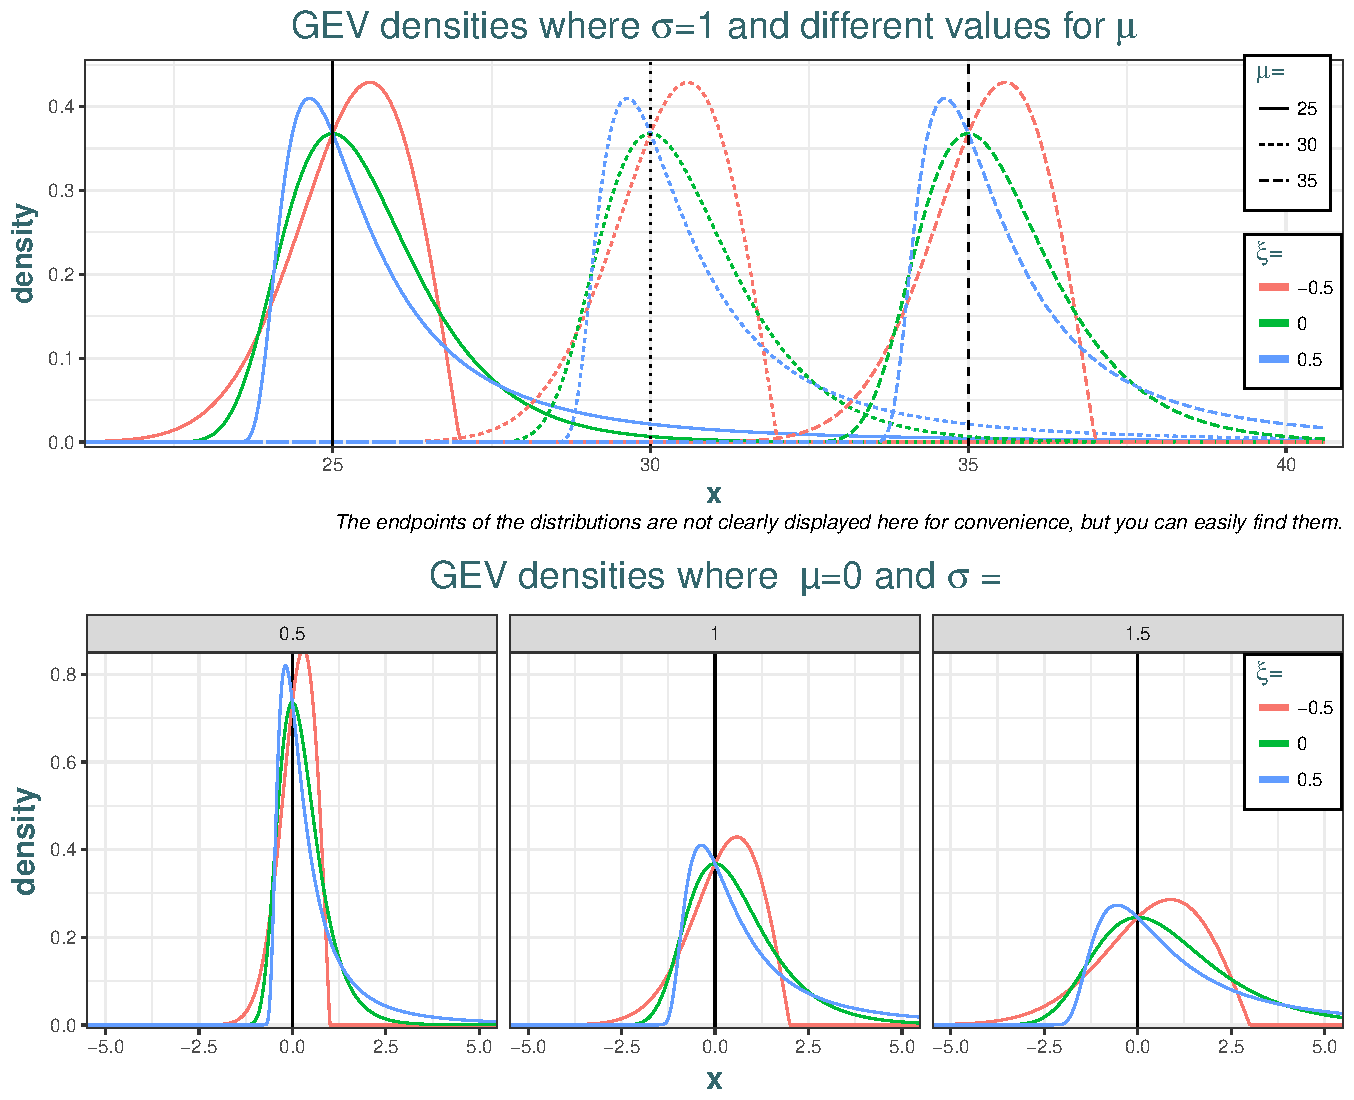
\includegraphics[width=\linewidth]{gevdif.pdf}\caption{GEV distribution for different values of the three parameters }\label{fig:gevdif}
\end{figure}


\section{Introduction of the Practical Analysis (section 6)}

\begin{figure}[!htb]
	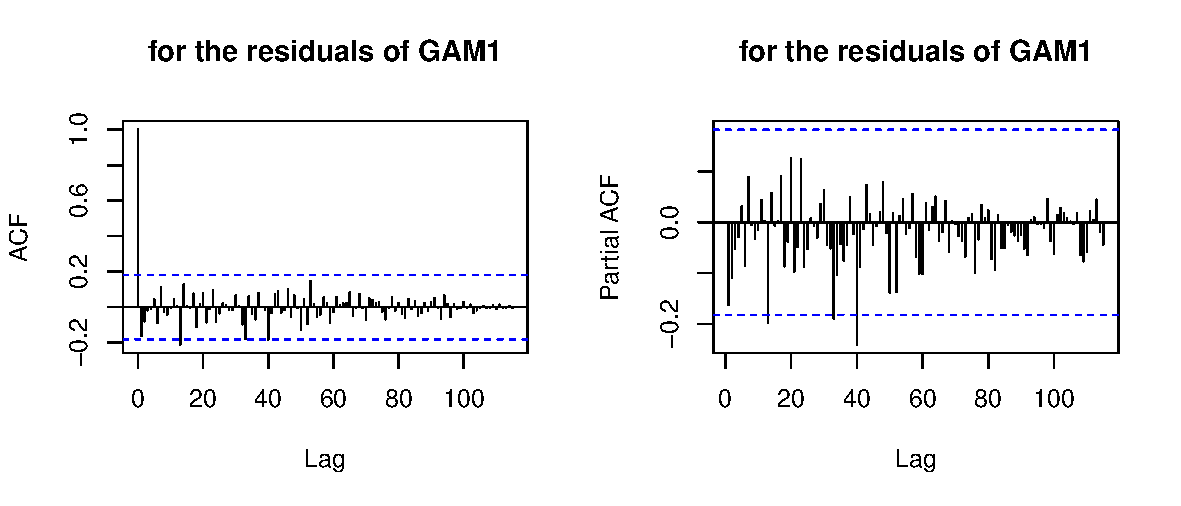
\includegraphics[width=\linewidth]{acfresgam.pdf}\caption{ACF and PACF for the residuals of the fitted GAM model with assumed independent errors }\label{fig:acfresgam1}
\end{figure}

\begin{table}[!htbp] \centering 
  \caption{compares models for the residuals of the GAM model based on AIC and BIC criterion. These criterion take into account the quality of fit (based on likelihood) but also a penalty term to penalize more complex models. } 
  \label{table:gamresid} 
\begin{tabular}{@{\extracolsep{5pt}} ccccc} 
\\[-1.8ex]\hline 
\hline \\[-1.8ex] 
& df & AIC & BIC \\ 
\hline \\[-1.8ex] 
Uncorrelated  & $4$ & $494.635$ & $505.650$ \\ 
AR(1)  & $5$ & $494.356$ & $508.124$ \\ 
MA(1) & $5$ & $493.706$ & $507.474$ \\ 
ARMA(1,1)  & $6$ & $492.511$ & $509.033$ \\ 
AR(2)  & $6$ & $495.133$ & $511.654$ \\ 
MA(2)  & $6$ & $494.698$ & $511.219$ \\ 
\hline \\[-1.8ex] 
\end{tabular} 
\end{table}


\begin{figure}[!htb]
\centering	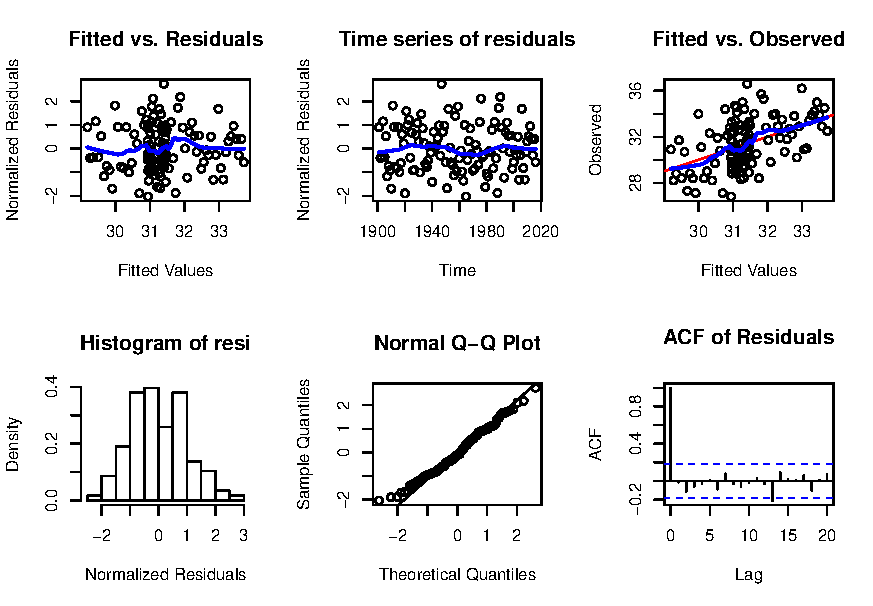
\includegraphics[width=.85\linewidth]{diagnogam.pdf}\caption{Diagnostics of the chosen GAM model with MA(1) errors, based on the residuals. }\label{fig:diagnogam}
\end{figure}


\begin{figure}[!htb]
\centering	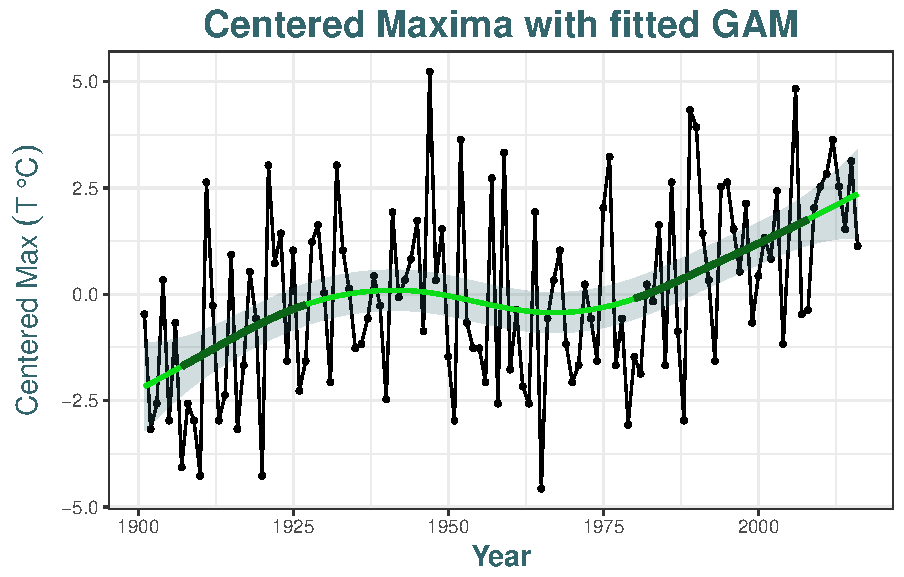
\includegraphics[width=.7\linewidth]{max_gam.pdf}\caption{Series of annual maxima together with the fitted GAM model (in green). Thicker lines indicate that the increase is significant for \underline{pointwise} confidence interval. Shaded area represent the "$95\%$" interval which looks quite narrow. }\label{fig:center_gam}
\end{figure}




\section{Analysis by GEV}


\begin{figure}[!htb]
\centering	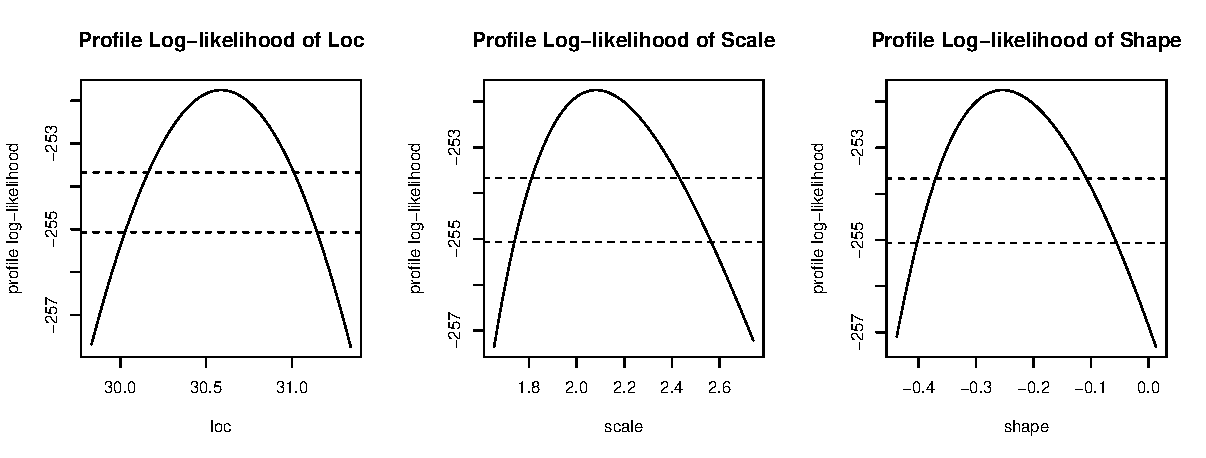
\includegraphics[width=.85\linewidth]{proflikpar.pdf}\caption{ The two horizontal dotted lines represent the 95$\%$ (above) and $99\%$ (below) confidence intervals when we take the intersection on the horizontal axis. }\label{fig:proflikpar}
\end{figure}



\iffalse
\begin{figure}
	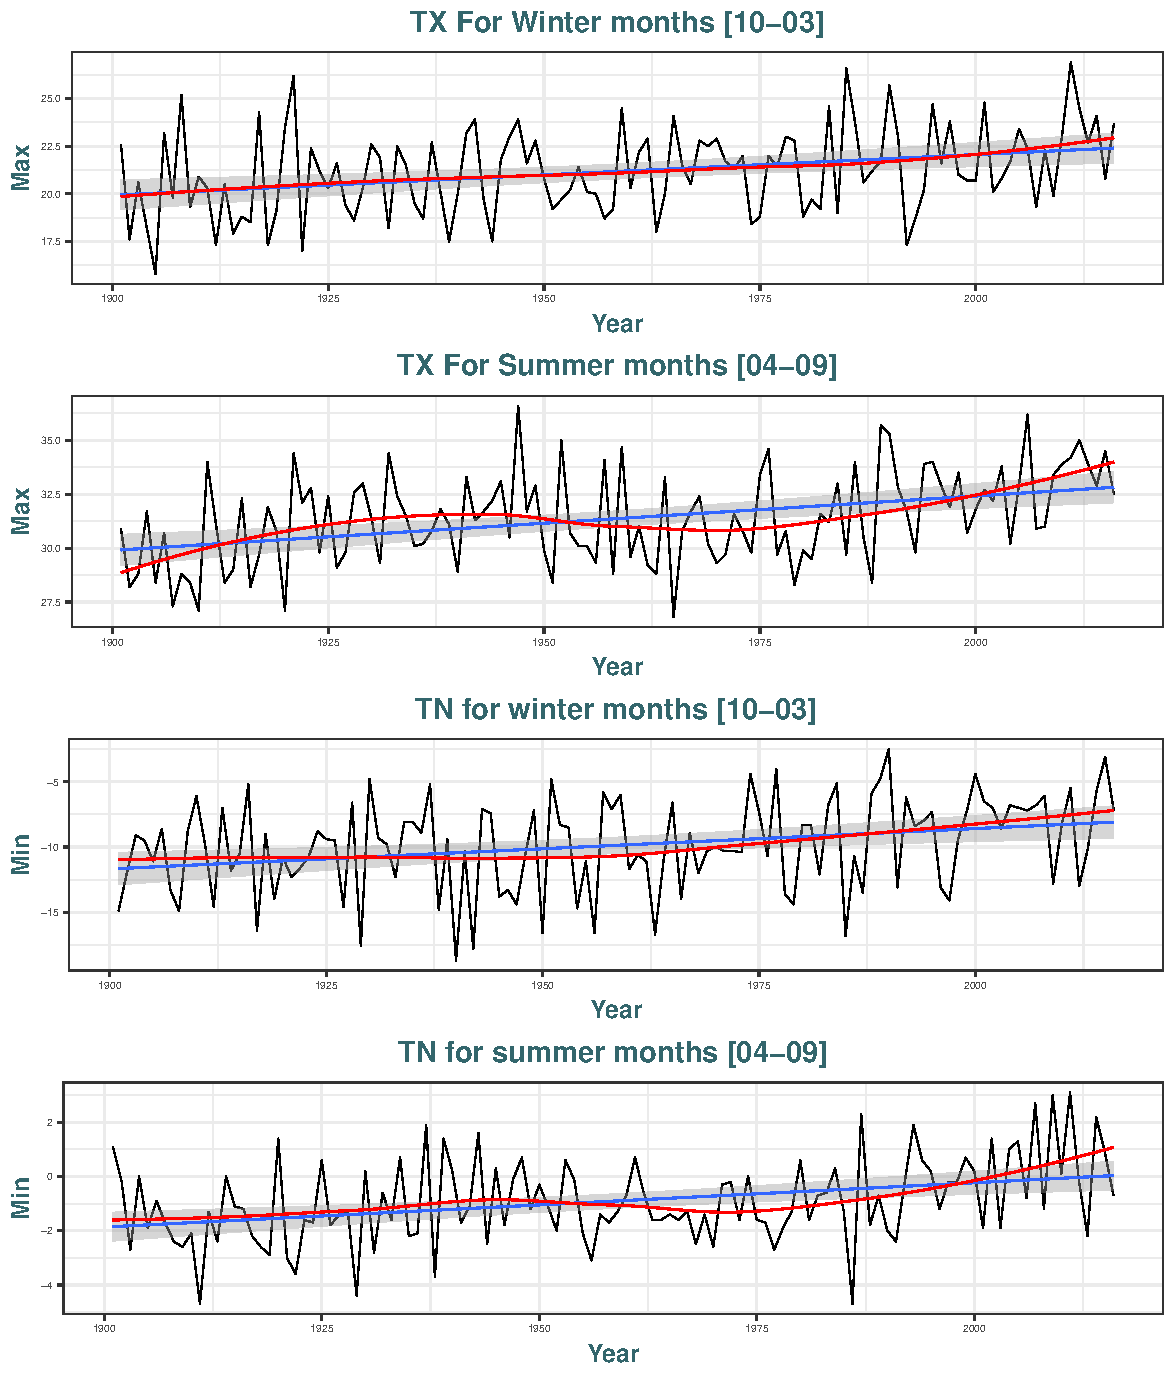
\includegraphics[width=.7\linewidth]{sumwint.pdf}\caption{First plot representing the \textbf{yearly} maxima (above) and minima (below) taking only the summer months (April to September) and winter months (October to March), shaded grey line around the linear trend represents its standard error. See how the polynomial trend (red line) also changes. Obv, TX for smummer and TN for winter are the same series as for the global serie}\label{seas4}
\end{figure}
\fi 


\iffalse
\begin{figure}[!h]
	\minipage{\textwidth}
	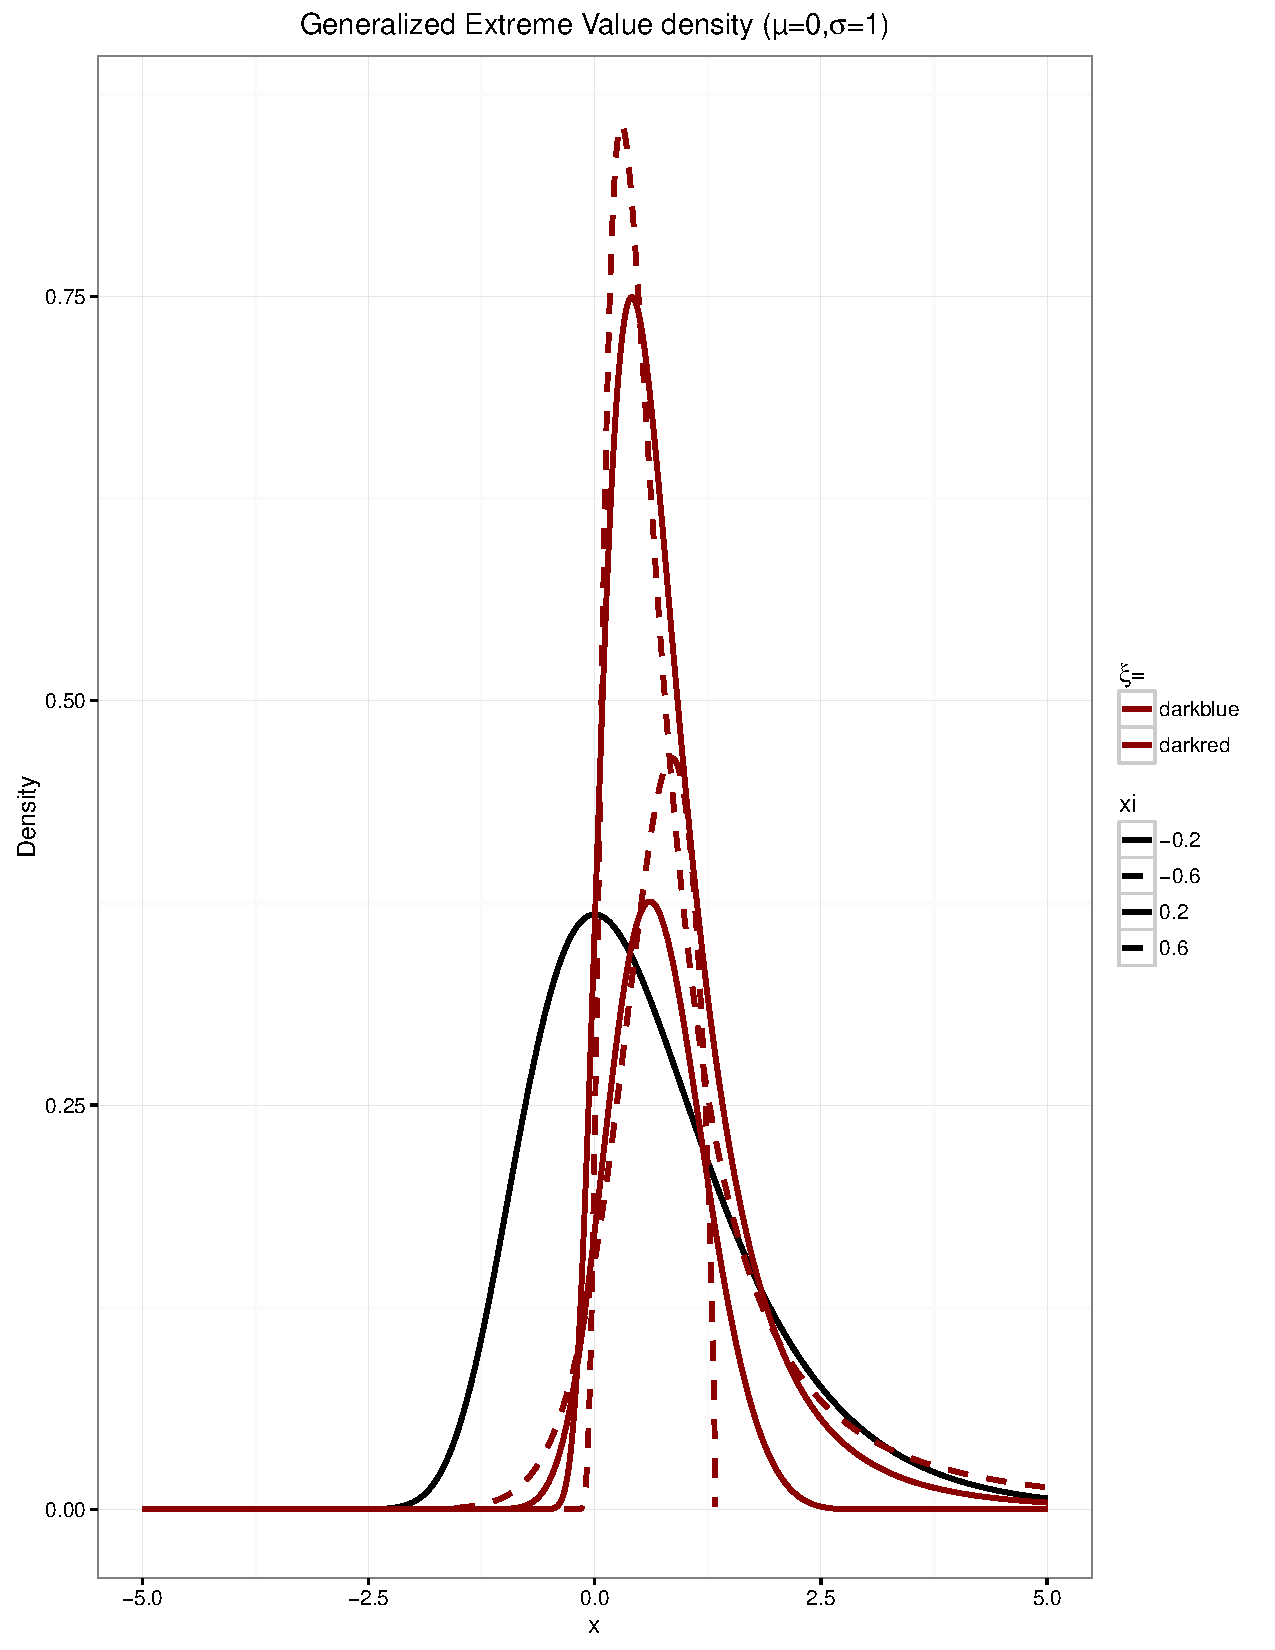
\includegraphics[width=\linewidth]{GEVV.pdf}
	\caption{ }\label{mcacls}
	\endminipage
\end{figure}
\begin{figure}[t!]
	$\begin{array}{rl}
	\multicolumn{2}{c}{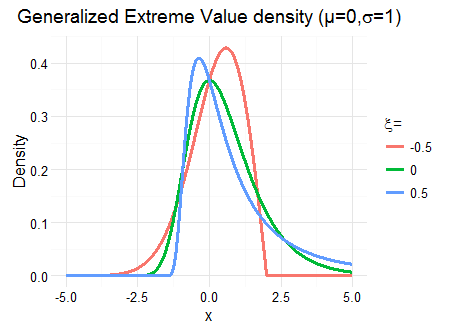
\includegraphics[width=0.85\textwidth]{GEV05.png}}\\
	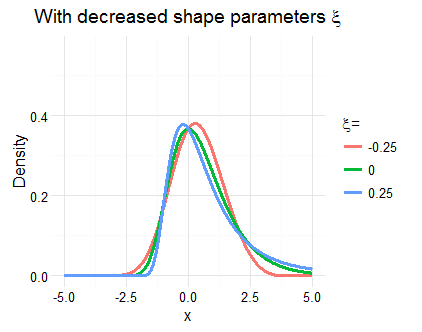
\includegraphics[width=0.5\textwidth]{GEV025.png} &
	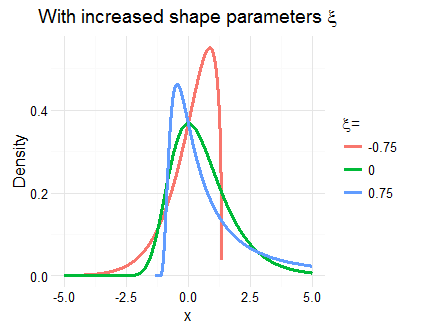
\includegraphics[width=0.5\textwidth]{GEV075.png}
	\end{array}$
	\caption{Representation of the GEV densities for various values of the shape parameter $\xi$ : $|\xi|=0.5$ (1) $|\xi|=0.25$, (2) and $|\xi|=0.75$ (3) for the Fréchet density [red], Weibull density [blue] while the Gumbel density [green] is kept fixed with $\xi=0$. }{\label{gevdens}}
\end{figure}
\fi 


\chapter{Github Repository Structure}\label{appgit}

The Github repository build for this thesis can be found on this address :

\begin{center}
\url{https://github.com/proto4426/PissoortThesis}
\end{center}

where the R package \textbf{\texttt{PissoortThesis}} is located. It has the following \textbf{structure} : 

\begin{itemize}
\item \textbf{/R/} : contains the scripts with all the functions that are made available through the package. The functions are located in the script by "category", i.e. 
\begin{itemize}
\item \textbf{1UsedFunc.R} : some functions created for the introduction, the stationary analysis of yearly maxima in GEV, analysis in POT, nonstationary analysis in GEV and POT,...
\item \textbf{BayesFunc.R} : functions created for the Bayesian Analysis, e.g. the Metropolis-Hastings algorithm and Gibbs Sampler (both stationary and nonstationary).
\item \textbf{BootstrapFunc.R} (not updated)
\item \textbf{NeuralNetsFunc.R} : functions slightly refined from \citet{cannon_flexible_2010} to allow for better outputs for the nonstationary analysis with NN.
\item \textbf{runExample.R} : contains the function allowing to run the Shiny applications directly through the package (put the name of the application in ' ' in the function to load the application). 
\end{itemize} 

The documentation of the functions are directly made through the package, by typing \texttt{?Function\_Name}.
\item \textbf{/Scripts-R/}

\begin{itemize}
\item \textbf{1GEV\_plots\_(chap1).R} and \textbf{1GEV\_ggplot\_(chap1).R} : contain the plots made for the chapter 1, but only te last latter scripts contain the code to construct the final plots (made with \texttt{ggplot2})
\item\textbf{1intro\_stationary.R} introduction and preprocessing +  descriptive analysis, stationary analysis of yearly maxima in GEV, analysis in POT, analysis with other time scale and with minima, ...
\item\textbf{1intro\_trends(splines).R} 
\item\textbf{1intro\_stationary.R} 
\item\textbf{1intro\_stationary.R} 
\item\textbf{1intro\_stationary.R} 
\item\textbf{1intro\_stationary.R} 
\item\textbf{1intro\_stationary.R} 
\item\textbf{1intro\_stationary.R} 
\item\textbf{1intro\_stationary.R} 
\end{itemize}


\item \textbf{/Shiny\_app\_visu/} (not updated)
\item \textbf{/data/}
\item \textbf{/inst/}
\item \textbf{/man/}
\item \textbf{/stan/}
\item \textbf{/vignettes/}
\end{itemize}
